\documentclass[10pt]{article}
\usepackage{pgf,tikz}
\usepackage{mathrsfs}
\usetikzlibrary{arrows}
\pagestyle{empty}
\begin{document}
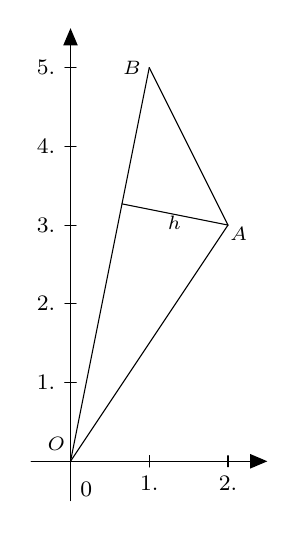
\begin{tikzpicture}[line cap=round,line join=round,>=triangle 45,x=1.0cm,y=1.0cm]
\draw[->,color=black] (-0.5,0.) -- (2.5,0.);
\foreach \x in {,1.,2.}
\draw[shift={(\x,0)},color=black] (0pt,2pt) -- (0pt,-2pt) node[below] {\footnotesize $\x$};
\draw[->,color=black] (0.,-0.5) -- (0.,5.5);
\foreach \y in {,1.,2.,3.,4.,5.}
\draw[shift={(0,\y)},color=black] (2pt,0pt) -- (-2pt,0pt) node[left] {\footnotesize $\y$};
\draw[color=black] (0pt,-10pt) node[right] {\footnotesize $0$};
\clip(-0.5,-0.5) rectangle (2.5,5.5);
\draw [line width=0.4pt] (2.,3.)-- (0.,0.);
\draw [line width=0.4pt] (0.,0.)-- (1.,5.);
\draw [line width=0.4pt] (1.,5.)-- (2.,3.);
\draw [line width=0.4pt] (0.6538461538461539,3.269230769230769)-- (2.,3.);
\begin{scriptsize}
\draw[color=black] (2.1371739255622675,2.8870972942641178) node {$A$};
\draw[color=black] (-0.17944410127952476,0.2237745287113123) node {$O$};
\draw[color=black] (0.7818735833282939,4.998844339140307) node {$B$};
\draw[color=black] (1.317689997699865,3.0289310510095335) node {$h$};
\end{scriptsize}
\end{tikzpicture}
\end{document}